\documentclass[10pt, oneside,english]{article}      
\usepackage{geometry}                       
\usepackage{graphicx}
\usepackage{amssymb}
\usepackage{authblk}
\usepackage{physics}
\usepackage{hyperref}
\usepackage{bm}
\geometry{a4paper}                                      



\title{\vspace{-1cm} MEK4470, Project description, transonic reentry in upper atmosphere}
\author{Trym Erik Nielsen}
\affil[1]{Department of Mathematics}
\affil[ ]{University of Oslo}
\renewcommand\Authands{, }
\date{\today}                         

\begin{document}
\maketitle
\section{Problem description, research questions}

Compressible fluid flow is an area of study that is greatly important to the field of aeronautical and astronautical engineering; in this project. We will look at the classical and often studied problem in transonic, compressible fluid flow, that of a spacecraft re-entering the atmosphere at high speed. Engineers study this problem in order to reduce damage on the spacecraft due to ablative effects from friction between the atmosphere and the skin of the vehicle, as well as analyze the stability of the spacecraft due to rotational moments, and the preseence of shockwaves.  

We can split our project into relevant numerical analysis questions of the underlying mathematics, as well as questions related to the underlying physics and dynamics of the proposed fluid flow. We will attempt in this project to answer the following questions concering the underlying physics of the proposed flow regime. 

\begin{itemize}
\item \textbf{How does the angle of attack affect the drag subjected to the vehicle?}
\item \textbf{How does the atmospheric conditions (i.e density, ambient pressure) affect the temperature of the leading edge of the vehicle?}
\item \textbf{How does the above affect the generation of shockwaves around the vehicle?}
\end{itemize}

We shall also attempt to answer the following questions concerning the underlying algorithms used in openFoam to analyze our proposed flow regime:

\begin{itemize}
    \item  \textbf{Does our selection of solver (rhoCentralFoam/sonicFoam) affect convergence towards a solution?}
    \item  \textbf{Does the solution converge both in space and time? for Mach number higher than 1?}
    \item \textbf{Does our solution for drag and maximum temperature agree with observed data?}
\end{itemize}

\clearpage
\section{Governing Equations}

The compressible form of the Navier Stokes equations can be expressed as:

\begin{displaymath}
    \pdv{\rho}{t} + \nabla \cdot (\rho \bm{U}) = 0
\end{displaymath}

\begin{displaymath}
    \pdv{\rho \bm{U}}{t} + \nabla \cdot (\rho \bm{U} \bm{U}) = \nabla p + \nabla \cdot \tau
\end{displaymath}

In the above equations, $\rho$ is the density of the fluid, $p$ is the pressure, and $\tau$ is the viscous stress tensor. The stress tensor $\tau$ can be expressed as 

\begin{displaymath}
    \tau = 2\, \mu\, dev(\bm{\underline{U}})
\end{displaymath}

where $dev(\bm{\underline{U}})$ is the deviatoric component of the deformation tensor, and $\mu$ is the dynamic viscosity of the fluid.


\section{Methodology: meshing and solver selection}

In the following figure, we can see a potential mesh for the flow problem, notice we have used the axis symmetric nature of the vehicle to reduce the computational complexity.

\begin{figure}[h!]
    \centering
    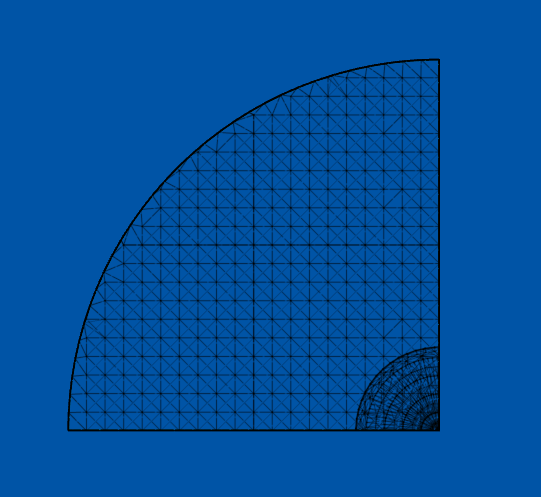
\includegraphics[width=0.5\linewidth]{figures/frontview_mesh}
    \caption{Front view of mesh}
    \label{fig:MeshFront}
\end{figure}        

We can see the denser lines of the vehicle geometry in the bottom right in \ref{fig:MeshFront}.

\begin{figure}[h!]
    \centering
    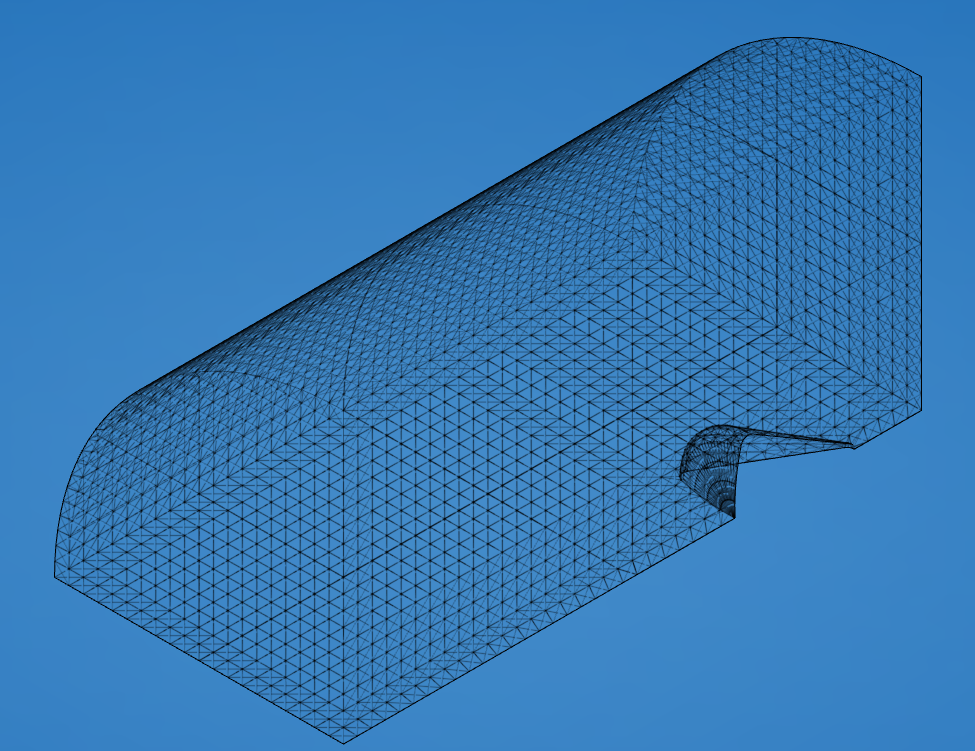
\includegraphics[width=0.5\linewidth]{figures/isometric_mesh}
    \caption{Isometric view of mesh}
    \label{fig:MeshIso}
\end{figure}   

Figure \ref{fig:MeshIso} shows the full quarter cylinder mesh domain in isometric view. The proposed mesh should help reduce the computational complexity, and therefore reduce the time needed to produce a converged solution.

For solver application in openFoam, we will attempt to solve our flow domain using both rhoCentralFoam and sonicFoam. sonicFoam uses the PISO algorithm, allowing for larger timesteps, wheras rhoCentralFoam solves the compressible flow regime using central schemes (hence the name), and flux limiters for solution stability. See the paper \href{https://cimec.org.ar/ojs/index.php/mc/article/viewFile/4231/4157}{High speed flow simulation using openfoam} for more information on the selected solvers. 

\section{Expected results}
We expect the angle of attack of the spacecraft relative to the direction of upstream fluid velocity to play a great affect in the temperature, the drag, as well as the shape of the shockwaves created. We expect convergence in time to be faster than convergence in space, due to the use of the PISO algorithm not requiring small $\delta t$ for stability. And we further expect a stiff problem with convergence difficulty for the higher initial Mach numbers in the flow. 

\end{document}   